\documentclass[10pt,a4paper,titlepage]{article}
\usepackage[utf8]{inputenc}

\usepackage{amsmath}
\usepackage{amsfonts}
\usepackage{amssymb}
\usepackage{graphicx}
\usepackage{float} % force figure to render inline location
\usepackage{enumitem} % apt install texlive-latex-extra 
\usepackage{anyfontsize} % custom fontsizes
\usepackage{titlesec} % custom section spacings
\usepackage{multirow} % merge table rows
\usepackage{vhistory} % revision table package
\usepackage{pdfpages}

\setlist[itemize]{noitemsep} % No spaces in itemize lists
\setlist[enumerate]{noitemsep} % No spaces in itemize lists
\setlist[description]{noitemsep} % No spaces in itemize lists
\titlespacing*{\subsubsection}{0pt}{8pt}{2pt}
\titlespacing*{\paragraph}{0pt}{3pt}{5pt}

\newcommand{\cpright}{\textsuperscript{\tiny\copyright}}

\setlength\parindent{0pt}

\begin{document}
	
	\begin{titlepage}
		
		\title{
			\fontsize{50}{12}\selectfont{\textsc{Lunar Rover}}\\
			\vspace{20pt}
			\fontsize{20}{12}\selectfont{\textsc{Software Project Management Plan}}\\
			\vspace{10pt}
			\large{Software Engineering \& Project} \\
			\vspace{20pt}
			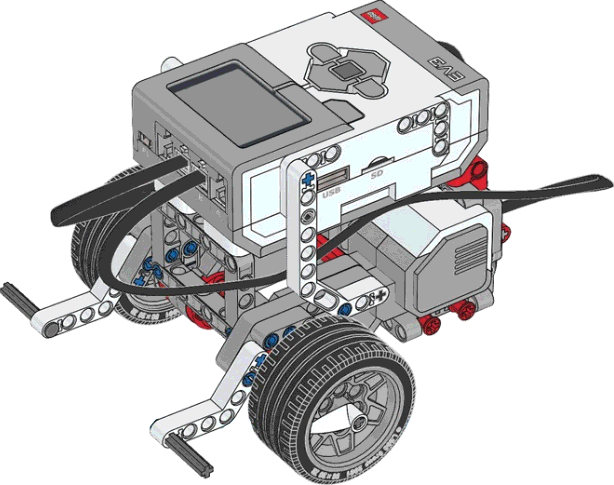
\includegraphics[width=200px]{title-page-ev3.png}					
		}
		\date{05/09/2017}
		\author{
			\bf{Team: PG-29} \\
			Benjamin Winding \\
			Kin Leong Lee \\
			Pavitterjeet Sidhu \\
			Phan Huy Nguyen \\
			Sean Hennessy \\
			Xiaoshan Chen \\
		}
		\maketitle
		
	\end{titlepage}
		 
	\tableofcontents	
	\listoffigures
	\listoftables
	
	
	\section*{Revision History}	
	\label{revtable}	
	\begin{tabular}{|p{2.1cm}|p{2.5cm}|p{2cm}|p{4.1cm}|}		
		\hline 
		\textbf {Name} & \textbf{Date} & \textbf {Version} &\textbf {Summary of Changes} \\ 
		\hline 
		\hline 		
	\end{tabular}

	\newpage
	
	\section{Introduction}
		%%%%%%weekly meeting template, prepared by Michael Sheng.  09/03/2007
\documentclass[11pt, a4paper]{article}
\usepackage{times}
\usepackage{ifthen}
\usepackage{amsmath}
\usepackage{amssymb}
\usepackage{graphicx}
\usepackage{setspace}

%%% page parameters
\oddsidemargin -0.5 cm
\evensidemargin -0.5 cm
\textwidth 15 cm
\topmargin -1.2 cm
\textheight 22 cm

\renewcommand{\baselinestretch}{1.1}\normalsize
\setlength{\parskip}{0pt}

\begin{document}


	
	\section{Introduction}
	\subsection{Purpose and Scope}
	The purpose of this project involves building a prototype rover capable of surveying a designated area automatically, developing a safe system for the client properly. The map shall be constructed  in real time as long as the robot starts the survey, showing lines, obstacles and current location of the robot. The final product is relies on the existing EV3 LEGO Mind-storms robot provided by the client. It is to be controlled via a remote location, but is required to automatically make decisions based on the environment around it. The final product shall should meet the requirements of client, which is included in the software specification document.
	
	\subsection{Assumptions and Constraints}
	\paragraph{}
	 Assumptions include:
	\begin{itemize}
		\item The group will contain 6 members throughout the project 
		\item Everyone will complete the assigned sections 
		\item Each member in the group are expected to spending 120 hours completing the project
		\item The functionalities of robot will be good during the client demonstrations
		
	\end{itemize}
	\paragraph{}
	
	Constraints include:
	\begin{itemize}
	\item The system is to be implemented using the EV3 LEGO Mind-storms kit supplied by the client.
	\item The embedded software on the rover is to be written in Java, using the LeJOS Ev3 library version:0.9.0
	\item The external code used in the system shall not exceed 10\%
	\item The build tool for compiling the software and deploying it to the system is ant. 
	\item The system will be implemented using the wireless technology WiFi over an encrypted WPA2 connection.
	\end{itemize}
	
	\subsection{Project Deliverables}
	The deliverables and due date of this project are list in the figure 1.
		\begin{figure}
		\centering
		\begin{tabular}{|p{8cm}|p{3cm}|}
	
			\hline 
			\textbf{Deliverables} &\textbf{Due Date} \\ 
			\hline 
				Software Requirement Specification 1st Draft & 22 Aug, 2017\\ 
			\hline 
				Software Project Management Plan 1st Draft & 5 Sep, 2017  \\ 
			\hline 		
				Milestone 1 demo specification finalize and sign agreement & 5 Sep, 2017 \\ 
			\hline 
				Milestone 1 demo & 12 Sep, 2017\\ 
			\hline 
				Milestone 2 demo specification finalize and sign agreement & 12 Sep, 2017 \\ 
			\hline 
				Software Design Document Draft & 3 Oct, 2017\\ 
			\hline 
				Milestone 2 demo & 3 Oct, 2017\\ 
			\hline 		
				User manual and instruction draft & 17 Oct, 2017\\ 
			\hline 
				Release final version of SRS, SPMP, SDD and user manual & 24 Oct, 2017\\ 
			\hline 
				Code free and product release & 24 Oct, 2017\\ 
			\hline 
				Final presentation & 31 Oct, 2017\\
			\hline
		\end{tabular} 
		\caption{The due date of project deliverables}
		\label{fig:tab Os Requirements}			
		\end{figure}

	\subsection{Evolution of the plan}
		\paragraph{}
	The changes to the management plan will happen when:
	\begin{itemize}
		\item the definition of task is changed
		\item the group is not able to finish the task before deadline
		\item the group complete the task ahead of deadline		
	\end{itemize}
	\paragraph{}
	The project manager will evaluate the performance when task is completed and will held a group meeting with group members to review issues. When the task is completed ahead of deadline, tasks whose deadline is in the future can be added in advance.

	
	
	
	
	



	
\end{document}

	\section{References}
		\begin{itemize}
	\item ‘A Guide to the Project Management Body of Knowledge’ 2013, 5th edn, Project Management Institute
	\item IEEE Recommended Practice for Software Requirements Specifications, IEEE Std 830-1998
	\item Google Java Style Guide, 2016, https://google.github.io/styleguide/javaguide.html
\end{itemize}
	\section{Definition}
		\begin{itemize}
	\item \textbf{SRS-}Software Requirements Specification
	\item \textbf{SPMP-}Software Project Management Plan
	\item \textbf{SDD-}Software Design Document
	\item \textbf{GUI-}Graphic User Interface
	\item \textbf{IDE-}Integrated Development Environment
\end{itemize}
	
	\section{Project Organisation}
		\subsection{The role and responsibilities}
The Software project team consists of Project manager, Documentation Manager, Testing Manager, IT Manager, Development Manager and Quality Manager. The team member’s role and responsibilities are listed as below.

\begin{itemize}
\item \textbf{Name: Pavitterjeet Sidhu}
\item Role: Project Manager
\item Responsibility: \\
1.	Planning all activities throughout the project life cycle, assigning each team member’s duties and monitoring their progress.\\
2.	To organise internal and client meetings.\\
3.	To ensure the project moving along on the right path and meet the deadline.
\item Reason:
Pavi has experience of lending a project. He is familiar with the project’s process model.
\end{itemize}

\newpage
\begin{itemize}
\item \textbf{Name: Benjamin Winding}
\item Role: Documentation Manager
\item Responsibility:\\
1.	To integrate team member’s documentation work and design project structure.\\
2.	To review team member’s document such as SPMP, SRS and SDD and ensure its the quality with acceptance level.
\item Reason:
Ben has experience of using latex and github. He can identify the issue of our latex file quickly and be familiar with using github to make a file structure.
\end{itemize}

\begin{itemize}
\item \textbf{Name: Kin Leong Lee}
\item Role: Testing Manager
\item Responsibility:\\
1.	To design a set of testing cases and testing scripts for Graphic User Interface and Robot’s functionalities.\\
2.	To review all testing results and write a testing report.
\item Reason:
Kin has experience of working in IT company and performed difference testing for software product. He is familiar with the testing process and building testing script.
\end{itemize}

\begin{itemize}
\item \textbf{Name: Xiaoshan Chen}
\item Role: IT Manager
\item Responsibility:\\
1.	To be responsible for the connection between EV3 robot and remote system.\\
2.	To handle and solve all the issues about using IDE.
\item Reason:
Shan has experience of working a IT company and responsible for IT support. She can handle difference IT problems and has experience of using intellij.
\end{itemize}

\begin{itemize}
\item \textbf{Name: Phan Huy Nguyen}
\item Role: Development Manager
\item Responsibility:\\
1.	To design the program structure and develop coding policies.\\
2.	To review all team member’s coding work including GUI, robot movement, robot sensors and path finding.
\item Reason:
Phan has software company working experience. He is familiar with the industry standard of coding.
\end{itemize}

\begin{itemize}
\item \textbf{Name: Sean Hennessy}
\item Role: Quality Manager
\item Responsibility:\\
1.	To identify all the risks of project throughout project life cycle.\\
2.	To plan the strategic to solve the project issues and ensue all the submitted works following the standard and good quality.
\item Reason:
Sean has experience of making budget plan for the project. He also studied project management course and has a skill to identify the risks of project.
\end{itemize}

The detail responsibilities for each team member shown as below:

\begin{table}[]
	\centering
	\caption{Responsibilities table}
	\label{my-label}
	\begin{tabular}{|l|l|l|l|l|l|l|}
		\hline
		Tasks/Members                                        & Pavi & Ben  & Issac & Shan & Phan & Sean \\ \hline
		\multicolumn{7}{|l|}{\textbf{Management}}                                                       \\ \hline
		Planning and Schedule                                & A\&R & I    & I     & I    & I    & I    \\ \hline
		Risk Management                                      & I    & I    & I     & I    & I    & A\&R \\ \hline
		Meeting Agenda                                       & R\&A & R    & R     & R    & R    & R    \\ \hline
		Meeting minutes                                      & R\&A & R    & R     & R    & R    & R    \\ \hline
		\multicolumn{7}{|l|}{\textbf{Documentation}}                                                    \\ \hline
		Documents (SRS, SPMP, SDD)                           & R    & R\&A & R     & R    & R    & R    \\ \hline
		Review Documents                                     & I    & R\&A & I     & I    & I    & I    \\ \hline
		\multicolumn{7}{|l|}{\textbf{Connection Management}}                                            \\ \hline
		Establish connection between robot and remote system & I    & I    & R     & R\&A & I    & I    \\ \hline
		Implement plugin to IDE and make it work             & I    & I    & I     & R\&A & I    & R    \\ \hline
		\multicolumn{7}{|l|}{\textbf{Software Development}}                                             \\ \hline
		Developing GUI                                       & R    & I    & R     & I    & R\&A & R    \\ \hline
		Developing Robot functionalities                     & I    & R    & I     & R    & R\&A & I    \\ \hline
		Integration                                          & R    & R    & I     & I    & R\&A & I    \\ \hline
		\multicolumn{7}{|l|}{\textbf{Testing}}                                                          \\ \hline
		Building Testing script                              & I    & R    & R\&A  & I    & R    & I    \\ \hline
		Acceptance Test                                      & R    & I    & R\&A  & R    & I    & R    \\ \hline
	\end{tabular}
\end{table}
\begin{itemize}
\item R(Responsible): Team member is responsible for this task
\item A(Accountable): Team member is responsible to assign the work to each group member
\item I(Informed): Team member will be informed when the task is completed
\end{itemize}
	\section{Risk Management}
		\documentclass[11pt, a4paper]{article}
\usepackage{times}
\usepackage{ifthen}
\usepackage{amsmath}
\usepackage{amssymb}
\usepackage{graphicx}
\usepackage{setspace}


\oddsidemargin -0.5 cm
\evensidemargin -0.5 cm
\textwidth 15 cm
\topmargin -1.2 cm
\textheight 22 cm

\renewcommand{\baselinestretch}{1.1}\normalsize
\setlength{\parskip}{0pt}

\begin{document}
		\subsection{Introduction}
		This risk management plan is implemented to identify and apply mitigation strategies to potential risks of the project. 
		The types of risks that will be identified will be those that may affect the health or safety of the personnel working on the project as well as 
		any risks to the expected delivery of the project. These risks will be categorised and given an impact and probability rating.
		\subsection{Identification}
			\subsection*{Types}
			There will be 5 risk categories identified. These are categories are follows: 
			\begin{itemize}
			\item Technology
			\item People
			\item Tools
			\item Requirements
			\item Estimation
			\end{itemize}	
			\subsection*{Priority convention}	
			There will be 3 main probability and impact  descriptors
			\begin{itemize}
			\item Low- probability:10-30\% , impact: 0-1 days project delay
			\item Medium - probabilty: 30-60\%, impact: 2-4 days project delay
			\item High- probability: 60-100\%, impact: >4 days project delay 
			\end{itemize}			
			
		\subsection{Analysis  and Planning}
			\subsection*{Technology Risks}
			\textbf{Robot or parts damaged or lost}\\
			Probability: Low\\
			Impact: High\\
			Strategy: If any parts or the whole robot is damaged or lost, the importance of the lost part is assessed by the team as a group. If necessary, the team must seek to collect funds in order to buy replacement parts.\\	
	
			\textbf{Wifi cannot handle code being sent to robot}\\
			Probability: Low\\
			Impact: High\\
			Strategy: Every week robot must be tested so that it can comply to commands via a wired cconnection

			\subsection*{People Risks}
			\textbf{Team members get sick at critical times}\\
			Probability: High\\
			Impact: Medium\\
			Strategy: Ensure any sick team members are encouraged to stay home in order to avoid spreading to other members. Project manager is to ensure that task assignment has some overlap in order to ensure there is at least one person able to work on critical sections.\\
			
			\textbf{Team members leave the course}\\
			Probability: Low\\
			Impact: High\\
			Strategy: Project manager to ensure that there is overlap in task assignment and that all team members have some expereience in every aspect of code.

			\subsection*{Tools}
			\textbf{University Github server no longer supported}\\
			Probability: Low\\
			Impact: High\\
			Strategy: Each team member to ensure that the project is pulled at least once per day on their machine. In the event of Github no longer being available, alternate version control methods such as SVN may be considered.

			\subsection*{Requirements}
			\textbf{Robot or parts damaged or lost}\\
			Probability: Low\\
			Impact: High\\
			Strategy:
			\subsection*{Estimation}
			\textbf{Robot or parts damaged or lost}\\
			Probability: Low\\
			Impact: High\\
			Strategy:
		
		\subsection{Monitoring}
\end{document}
	\newpage
	\section{Process Model}
		\documentclass[a4paper]{article}

%% Language and font encodings
\usepackage[english]{babel}
\usepackage[utf8x]{inputenc}
\usepackage[T1]{fontenc}

%% Sets page size and margins
\usepackage[a4paper,top=3cm,bottom=2cm,left=3cm,right=3cm,marginparwidth=1.75cm]{geometry}

%% Useful packages
\usepackage{amsmath}
\usepackage{graphicx}
\usepackage[colorinlistoftodos]{todonotes}
\usepackage[colorlinks=true, allcolors=blue]{hyperref}


\begin{document}


\section{Process model}

In this project, we are following agile process development model as shown in figure \ref{fig:process_model} because this project requires adaptive planning along with evolutionary development and continuous improvement. The initial phase of the project is focused on gathering the software requirement.There will be two official milestones and several internal project team milestones, in order to deliver the product on time. Project deliverables are divided into sub-activities and for each activity a development cycle will be followed which will include different phases such as design, development, testing, review and improvement.
\paragraph{} Agile process development model provides high customer satisfaction due to continuous delivery of the software modules and ensures the high quality software development. This model has advantages such as no planning is required to start the project as compared to other traditional software development models such as water fall in which project team makes strict promises to the client by doing requirement analysis and planning. This model is very easy to manage and provides great flexibility to the project team and client.

\begin{figure}
\centering
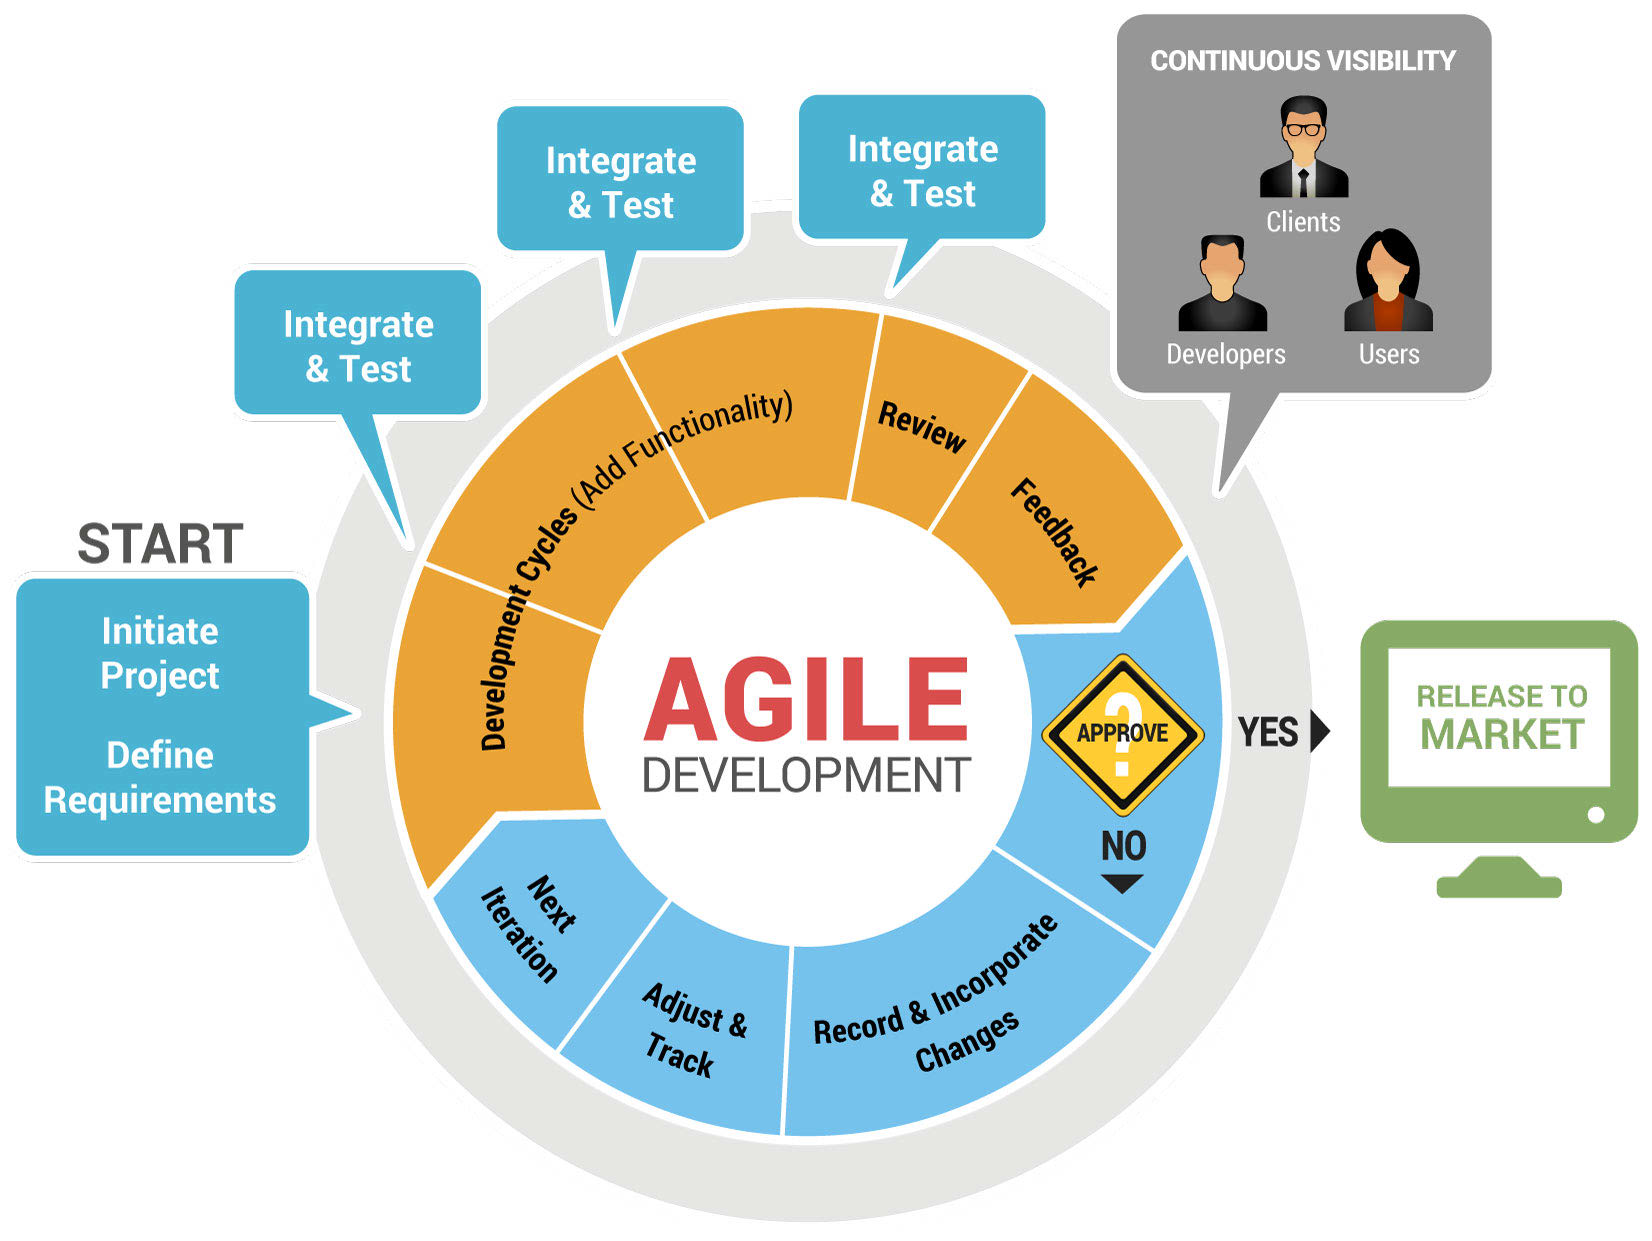
\includegraphics[width=0.9\textwidth]{process_model.png}
\caption{\label{fig:process_model}Agile process model diagram}
\end{figure}


\end{document}

	\section{Work Plan}
		\subsection{Work Activities}
	\subsubsection{Software Requirement Specification}
	\begin{itemize}
		\item SRS-T001: SRS Draft
		\begin{itemize}
			\item SRS-T001-1: Brainstorming meeting for ideas.
			\item SRS-T001-2: Understand and develop user requirement.
			\item SRS-T001-3: Define product features and functional requirement.
			\item SRS-T001-4: Develop external interface and non-functional requirements.
			\item SRS-T001-5: SRS draft finalization meeting.
		\end{itemize}
		\item SRS-T002: SRS Final Version
		\begin{itemize}
			\item  SRS-T002-1: Revise SRS draft following client's recommendations after SRS draft presentation meeting.
			\item  SRS-T002-2: Keep track client requirements change every weeks.
			\item  SRS-T002-3: Team review meeting before release official SRS document.
		\end{itemize}
	\end{itemize}

	\subsubsection{Software Product Management Plan}
	\begin{itemize}
		\item SPMP-T001: SPMP Draft
		\begin{itemize}
			\item SPMP-T001-1: Brainstorming meeting for ideas.
			\item SPMP-T001-2: Develop project organization, specific role and responsibility for each member in this project.
			\item SPMP-T001-3: Develop risk management plan.
			\item SPMP-T001-4: Analysis team characteristics and select appropriate process model.  
			\item SPMP-T001-5: Create working plan based on current SRS, process model and team capacity.
			\item SPMP-T001-6: SPMP draft finalization meeting.
		\end{itemize}
		\item SPMP-T002: SPMP Final Version
		\begin{itemize}
			\item  SPMP-T002-1: Revise SPMP draft following client's recommendations after SPMP draft presentation meeting.
			\item  SPMP-T002-2: Weekly update if there is with any change in process model, resources, development plan etc.
			\item  SPMP-T002-3: Team review meeting before release official SPMP document.
		\end{itemize}
	\end{itemize}

	\subsubsection{Software Design Document}
	\begin{itemize}
			\item SDD-T001: System Design
			\begin{itemize}
				\item SDD-T001-1: Develop system overview of product.
				\item SDD-T001-2: Define system components base on system overview.
				\item SDD-T001-3: System components design details for each component
			\end{itemize}
			\item SDD-T002: GUI Design
			\begin{itemize}
				\item SDD-T002-1: Analyst user requirements and system features.
				\item SDD-T002-2: Define GUI appropriate with each features.
				\item SDD-T002-3: Create the mock-GUI and test it feasibility and user experience.
			\end{itemize}
			\item SDD-T003: SDD Final Version
			\begin{itemize}
				\item  SDD-T003-1: Revise SDD draft following client's recommendations after SDD draft presentation meeting.
				\item  SDD-T003-2: Weekly update if there is with any change in requirements, features which need to be reflect into system design, GUI design etc.
				\item  SDD-T003-3: Team review meeting before release official SDD document.
			\end{itemize}
	\end{itemize}

	\subsubsection{Implementation}
	\begin{itemize}
		\item IMP-T001: Prototyping
		\begin{itemize}
				\item IMP-T001-1: Create simple manual control with UI.				
				\item IMP-T001-2: Create autonomous controller make robot move randomly with human control.
				\item IMP-T001-3: Enhance from IM-T001-2 make robot move follow a track to test color sensor.
				\item IMP-T001-4: Enhance from IM-T001-2 make robot automatically moving while detect and avoid obstacle. 
		\end{itemize}
		\item IMP-T002: GUI Implementation
		\begin{itemize}
				\item IMP-T002-1: Create GUI from mock-up design of SDD-T002.
				\item IMP-T002-2: Integration prototyping with new GUI.
				\item IMP-T002-3: Implement user input feature on GUI. Allow user to manually add new information such as NGZ, destination, landing site etc.
		\end{itemize}
		\item IMP-T003: Implement autonomous mode.
		\begin{itemize}
				\item IMP-T003-1: Implement path finding algorithm.
				\item IMP-T003-2: Enhance IMP-T001-3 and IMP-T001-4 so that robot can recognize and follow the track.
				\item IMP-T003-3: Enhance IMP-T001-3 and IMP-T001-4 so that robot can recognize physical obstacle, NGZ, cratters etc. 
				\item IMP-T003-3: Implement area map survey strategy by moving zig-zag while detect and avoid obstacles, NGZ, cratters etc.
		\end{itemize}
		\item IMP-T004: Implement manual control mode.
		\begin{itemize}
				\item IMP-T004-1: Implement warning and confirmation when user control robot into danger region.
				\item IMP-T004-2: Implement emergency stop feature.
				\item IMP-T004-3: Implement autonomous/manual switch.
		\end{itemize}
		\item IMP-T005: Map Display and Construction.
		\begin{itemize}
			\item IMP-T005-1: Display import map xml info onto GUI-MAP.
			\item IMP-T005-2: Display new informations return from sensor on GUI-MAP.
			\item IMP-T005-3: Display warning on GUI-MAP when robot move into danger region.
			\item IMP-T005-4: Implement export result survey xml map.
		\end{itemize}
		\item IMP-T006: Team final review.
		\begin{itemize}
			\item IMP-T006-1: Each member review all implemented features.
			\item IMP-T006-2: Final review meeting and collect team features feedback.
			\item IMP-T006-3: Make change base on feedback.
		\end{itemize}
	\end{itemize}

	\subsubsection{Testing}
	\begin{itemize}
		\item Test-T001: Unit Test.
		\begin{itemize}
				\item Test-T001-1: Create unit test for all major computation component.
				\item Test-T001-2: Regular review and make test case up to date.
		\end{itemize}
		\item Test-T002: Integration Test.
		\begin{itemize}
				\item Test-T002-1: Define test cases and test-acceptance criteria base on requirement and scope define in SRS.
				\item Test-T002-2: Meeting with client and finalize all test cases.
				\item Test-T003-3: Perform test product functionalities base on defined test cases while implement process.
				\item Test-T003-4: Keep track all change in requirement and update corresponding test cases.
				\item Test-T003-5: Recording all fail tests and keep track along side with development process.
		\end{itemize}
	\end{itemize}

	\subsubsection{User Manual}
	\begin{itemize}
		\item UM-T001: Define user manual structure.
		\begin{itemize}
				\item UM-T001-1: Team brainstorming for user manual ideas.
				\item UM-T001-2: Create user manual draft.
				\item UM-T001-3: Present and get feedback from clients.
		\end{itemize}
		\item UM-T002: Finalize user manual. 
		\begin{itemize}
				\item UM-T001-1: Review client feedback and revise user manual.
				\item UM-T002-2: Team meeting and release final version.
		\end{itemize}
	\end{itemize}

	\subsubsection{Release}
	\begin{itemize}
		\item RL-T001: Pre-Relase
		\begin{itemize}
			\item RL-T001-1: Run over all test case define in Test-T001 and Test-T002.
			\item RL-T001-2: Review and check is there any existing bug.
			\item RL-T001-3: Fix all fail test cases and existing bug. 
		\end{itemize}
		\item RL-T002: Create review checklist.
		\item RL-T003: Go over release checklist and deploy final product to client.
	\end{itemize}
	
	
\subsection{Milestone}
	\subsubsection{Internal Milestone}
		\begin{itemize}
			\item IMS-001: Robot manual control with basic movement.
			\begin{itemize}
				\item Due Date: End of week 3.
				\item Description:
				\begin{itemize}
					\item Simple GUI with buttons : Up, Down, Left, Right, Stop.
					\item Robot move as expected when use control button on GUI.
				\end{itemize}
			\end{itemize}
			\item IMS-002: Software Requirement Specification Draft.
			\begin{itemize}
				\item Due Date: End of week 4.
				\item Description:
				\begin{itemize}
					\item Have first draft of SRS document follow SRS template with all sections in detail.
					\item Document must be in LaTEX file.
					\item Document manager must perform proof-reading over whole document and edit spelling, grammar, formating mistake if any.
				\end{itemize}
			\end{itemize}
			\item IMS-003: Software Project Management Plan Draft
			\begin{itemize}
				\item Due Date: End of week 6.
				\item Description:
				\begin{itemize}
					\item Have first draft of SPMP document follow SPMP template with all sections in detail.
					\item Document must be in LaTEX file.
					\item Document manager must perform proof-reading over whole document and edit spelling, grammar, formating mistake if any.
				\end{itemize}
			\end{itemize}
			\item IMS-004: Mock-up of final GUI
			\begin{itemize}
				\item Due Date: End of week 6.
				\item Description:
				\begin{itemize}
					\item Finish GUI design with all GUI component which user need to finish their mission.
					\item Go through SRS user requirement, system features make sure all requirement can perform easy on GUI.
					\item Some buttons, features or component on GUI may not working since it just placeholder. 
				\end{itemize}
			\end{itemize}
			\item IMS-005: Software Design Document Draft
			\begin{itemize}
				\item Due Date: End of week 8.
				\item Description:
				\begin{itemize}
					\item Have first draft of SPMP document follow SPMP template with all sections in detail.
					\item Document must be in LaTEX file.
					\item Document manager must perform proof-reading over whole document and edit spelling, grammar, formating mistake if any.
				\end{itemize}
			\end{itemize}
			\item IMS-006: Robot autonomous survey mode
			\begin{itemize}
				\item Due Date: End of week 9.
				\item Description:
				\begin{itemize}
					\item Robot can automatically move inside survey area.
					\item Robot can detect and avoid obstacle, cratter, NGZ and avoid them.
					\item Robot can collect sensor data and display it on GUI-Map.
					\item Robot can move to point define by user.
					\item Robot can move follow track.
				\end{itemize}
			\end{itemize}
			\item IMS-007: Finish final GUI functionalities
				\begin{itemize}
				\item Due Date: End of week 10.
				\item Description:
				\begin{itemize}
					\item Every function on GUI work as define in SDD user interface section.
				\end{itemize}
			\end{itemize}
			\item IMS-008: Integration and Testing
			\begin{itemize}
				\item Due Date: End of week 11.
				\item Description:
				\begin{itemize}
					\item Integrate manual control mode and autonomous mode in to GUI.
					\item Verify all functionalities still working as expected and match with requirement in SRS document.
					\item Switch between manual/autonomous without any problem.
					\item Robot can complete survey in less than 20 minutes and return to landing site.
				\end{itemize}
			\end{itemize}
			\item IMS-009: Prepare for final presentation with client.
			\begin{itemize}
				\item Due Date: End of week 12.
				\item Description:
				\begin{itemize}
					\item All remaining must be solve.
					\item All test case must pass.
					\item Code review already perform and have a clear code base with sufficient up to date comment.
					\item Final code must be submit before code freeze deadline.
					\item Slide or Postcard must ready if there is required them.
				\end{itemize}
			\end{itemize}
		\end{itemize}
	\subsubsection{Client Official Milestone}
		\begin{itemize}
			\item OMS-001: Client Official Milestone 1 Demo.
			\begin{itemize}
				\item Due Date: End of week 7.
				\item Description:
				\begin{itemize}
					\item Finish GUI design with all GUI components which user need to finish their mission.
					\item Robot movement display correct on Map-GUI.
					\item Robot can move randomly and avoid obstacles and NGZ.
					\item Some buttons, features or component on GUI may not working since it is just placeholder. 
				\end{itemize}
			\end{itemize}
			\item OMS-002 : Client Official Milestone 2 Demo.
			\begin{itemize}
				\item Due Date: End of semester break.
				\item Description:
				\begin{itemize}
					\item Robot can move survey the area with effective strategy such as move cycle or zig-zag.
					\item User can manual define NGZ and robot can recognize NGZ, obstacle, crater to avoid them while survey.
					\item New informations of survey area are display in real-time on GUI-Map.
				\end{itemize}
			\end{itemize}
		\end{itemize}
	
	\subsection{Work Breakdown Structure}
The Fig.\ref{work-breakdown-structure} shows a work breakdown structure of this project. This project consists of 5 difference phases: Verfication of requirement, Project management plan development, Software development, Testing and product release. 
	\begin{figure}[H]
		\centering
		\hspace*{-1.3in}
		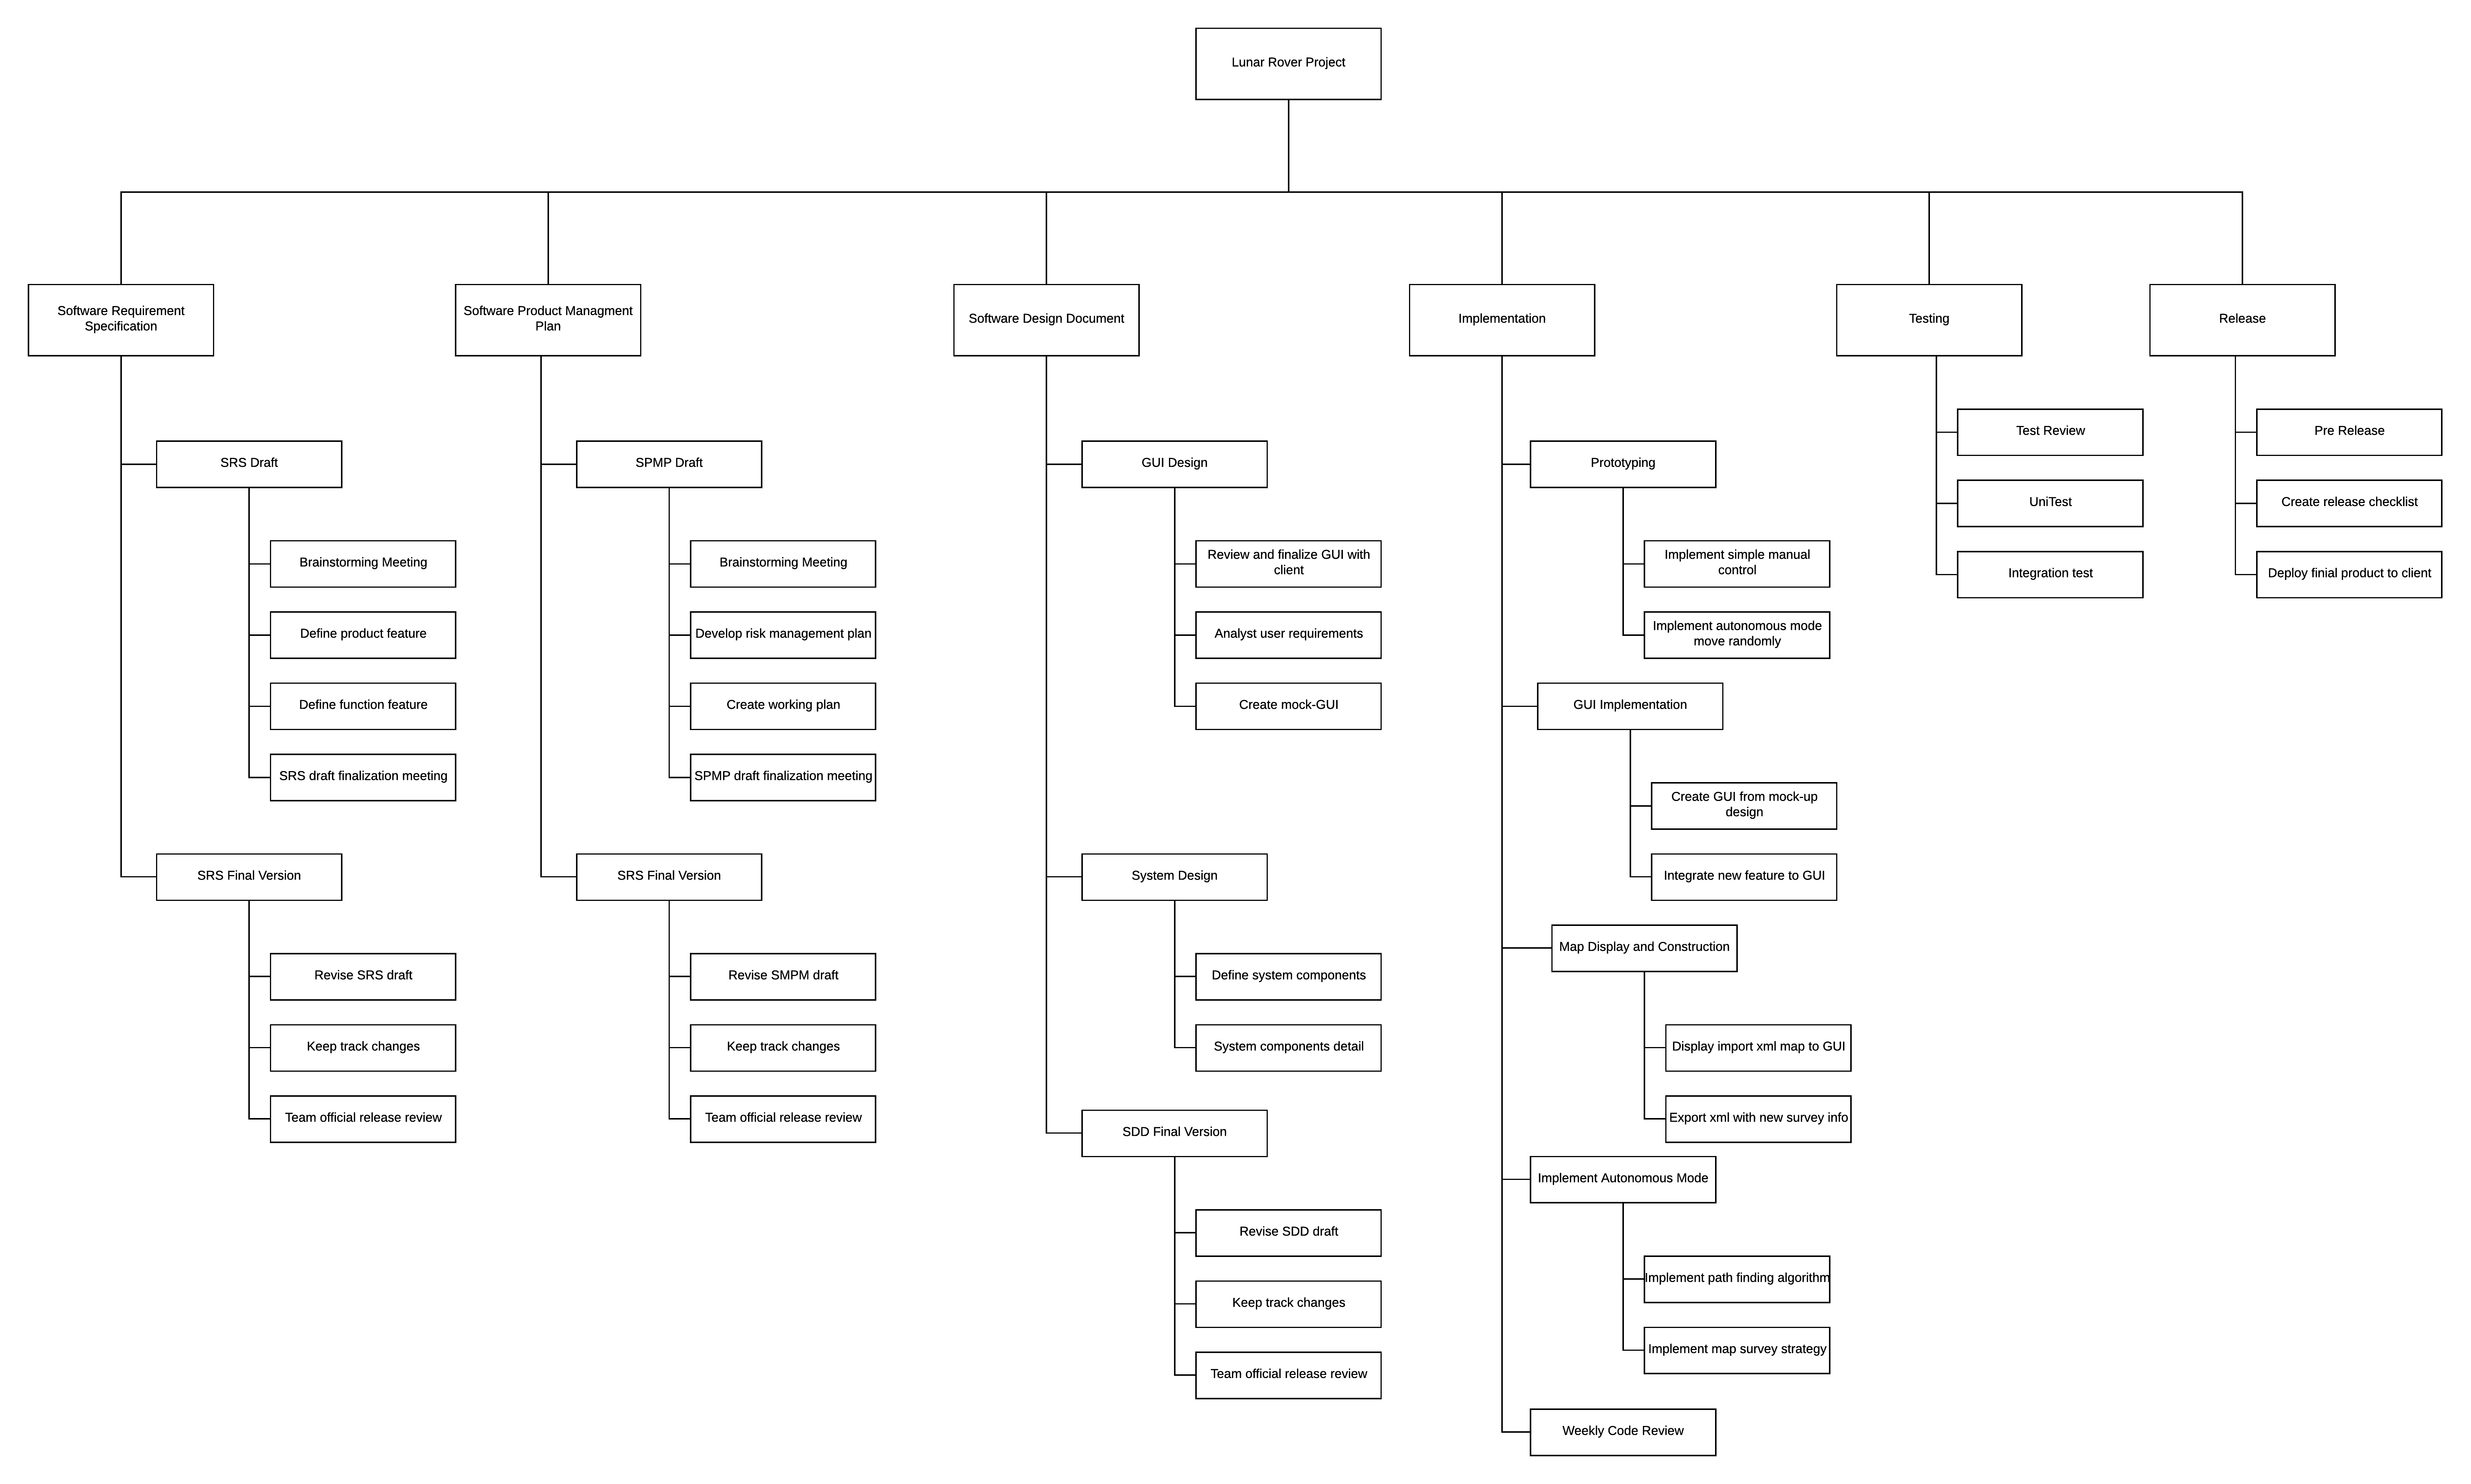
\includegraphics[width=1.5\linewidth]{WorkBreakDown_s.PNG}  % created using www.draw.io
		\caption{Work Breakdown Structure}
		\label{work-breakdown-structure}
	\end{figure}
\subsection{Schedule Allocation}
\subsubsection{Task schedule}
The task scheduling will be shown in detail by the Gantt chart below. In summary, the Gantt chart will indicate which team member has responsibility for a task. The time allocation for each task with a specific  deadline. Tasks can work in parallels are also visualize and can easy to find in the chart.     
\subsubsection{Major Task and Deadline Time}
	\begin{tabular}{|p{3cm}|p{8cm}|}
		\hline 
		\textbf{Deadline Time} &\textbf{Task name} \\ 
		\hline 
			Week 5 & Software Requirement Specification Draft\\ 
		\hline 
			Week 7 & Software Project Management Plan Draft\\ 
		\hline 		
			Week 7 & Milestone 1 demo specification finalize and sign agreement\\ 
		\hline 
			Week 8 & Milestone 1 demo\\ 
		\hline 
			Week 8 & Milestone 2 demo specification finalize and sign agreement\\ 
		\hline 
			Week 9 & Software Design Document Draft\\ 
		\hline 
			Week 9 & Milestone 2 demo\\ 
		\hline 		
			Week 11 & User manual and instruction draft\\ 
		\hline 
			Week 12 & Release final version of SRS, SPMP, SDD and user manual\\ 
		\hline 
			Week 12 & Code free and product release\\ 
		\hline 
	\end{tabular} 


	\newpage
	\section{Supporting Plans}
		\subsection{Configuration Management Plan}
This software project consists of 5 official documents including SRS, SPMP, SDD, Testing report and User Manuel), meeting agenda and minutes, and software for operating EV3 robot. All these configuration items’ standards are developed by documentation manager and monitored by quality manager. All team members are responsible for following this configuration standard during the whole project life cycle. The detail of software and testing components will be mentioned in SDD document and testing report.

\subsubsection{GitHub Repository structure and Configuration control}
The repository structure is built based on the component of the project. The highest level of repository is Code and Documentation. 
\begin{itemize}
	\item \texttt{\detokenize{...\2017-S2-SEP-PG29\Documentation}}
	\item \texttt{\detokenize{...\2017-S2-SEP-PG29\Code}}
\end{itemize}
The detail GitHub Repository structure is shown on fig.\ref{fig:GITHUB repository}.

\begin{figure}[H]
	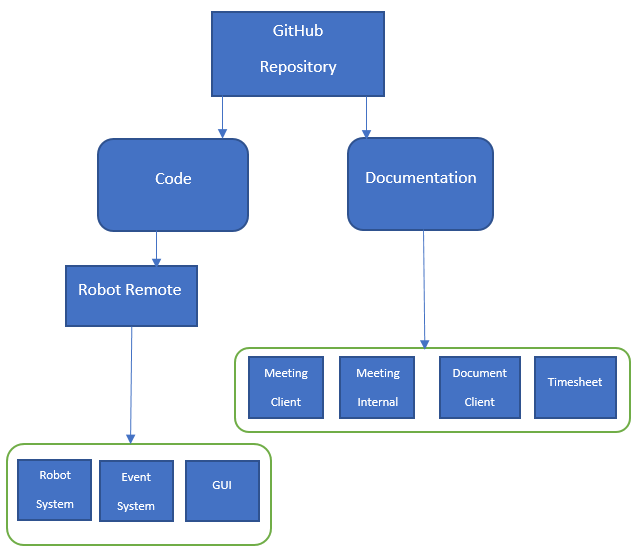
\includegraphics[width=\linewidth]{GIT.PNG}  % created using www.draw.io
	\caption{GITHUB repository}
	\label{fig:GITHUB repository}				
\end{figure}

There are three configuration directories which have special control for team members to edit. The Software components are not included in this section and will be discussed in detail on SDD document.\\
The lists of configuration control are shown as below:\\

\textbf{Library control:}\\
This library directory is for development purpose. There shall allow to store jar file only. No other file format is allowed. Team members are require to get the approval from development manager to add new jar file.\\ 
\begin{itemize}
	\item \texttt{\detokenize{...\Code\UiRemote\lib}}
\end{itemize}
\textbf{Media control:}\\
Those directory contain png file only. No other file format is allowed. Team members can feel free to add any png file for development or development purpose. Team members shall commit the change with proper message to indicate which files they are added.

\begin{itemize}
	\item \texttt{\detokenize{...Code\UiRemote\src\RobotRemote\UI\Views}}
	\item \texttt{\detokenize{...Documentation\Views}}
\end{itemize} 
\textbf{Documentation control:}\\
Those directories contain tex and pdf file only. Team members are not allowed to add any file in those directories.
Only documentation manager can add new file to those directories

\begin{itemize}
	\item \texttt{\detokenize{...Documentation\SRS}}
	\item \texttt{\detokenize{...Documentation\SPMP}}
	\item \texttt{\detokenize{...Documentation\SDD}}
\end{itemize}

\subsubsection{Configuration Naming System and version control}
Any draft of configuration items shall be followed as below naming standards:
\begin{itemize}
	\item \texttt{\detokenize{<Title>_<version>.<extension>}}\\
      		\texttt{\detokenize{For examples: SRS_v0.9.tex}}
	\item The Final version is v1.0. The draft version will be named as v0.1-v0.9.
	\item The modified date for each sub-version shall be mentioned in revision history table which is included into documents.\\
\end{itemize}

The examples of revision history for SRS-v0.9.tex is shown on Table.\ref{my-labelxxxx} :\\

\begin{table}[]
	\centering
	\caption{Revision history example}
	\label{my-labelxxxx}
	\begin{tabular}{|l|l|l|l|}
		\hline
		Name      & Date      & Version & Summary of Changes           \\ \hline
		1st Draft & 21/8/2017 & 0.9.1   & Initial Draft                \\ \hline
		2nd Draft & 22/8/2017 & 0.9.2   & Identification numbers added \\ \hline
	\end{tabular}
\end{table}


The revision table for final version shall include all the change for each version. After final version released, any change is required a change request which is mentioned in section 8.3.\\


The meeting agenda and meeting minutes shall follow as below naming system:\\
\texttt{\detokenize{<Title>_<Type>_<week>.<extension>}}\\
\begin{itemize}
\item Title: Agenda or Minutes
\item Type: Client or Internal
\end{itemize}
\texttt{\detokenize{For example: agenda_client_week3.tex, minutes_internal_week3.tex}} \\\\
Usually, there are only one client meeting and internal group meeting per week. If there are any emergency meeting, the date should be included.\\\\
\texttt{\detokenize{For example: agenda_internal_week3_17082017.tex}}\\
\texttt{\detokenize{The date format shall be <days><months><year>}}\\

\subsubsection{Change request handling}
There are two types change request handling. Documentation and Software change request handling.\\\\
\textbf{Documentation:}\\
The Documents will be divided by documentation manager into difference sub-tasks for each team member to edit their own parts. 
\begin{itemize}
\item Team members can make any change on their own part before the final version release. 

\item Team members is required to edit the revision table to record their change on the document. 

\item The documentation review meeting will be held by documentation manager to review all the changes on the document before releasing final version.

\item The change on Final version's document is not allowed without discussion in another new review meeting. 
\end{itemize}
\textbf{Software:}
\begin{itemize}
\item Team member must need to create new branch in github repository to make a change or add new function on software. 
\item The change on this branch must not affect master branch.
\item Regular software review meeting will be held by development manager to review all the team member’s work and discuss the potential issue before merging the work to master branch.
\end{itemize}

\newpage

% 8.2
% Documentation plan
% List the documents to be prepared. Give details on the document template to be used (whereappropriate). Describe the preparation and review process for documents.

\subsection{Documentation Plan}
The documentation plan involves several key documents and revision processes that ensure the quality of the overall project is kept at a high level.

\subsubsection{SRS}
The Software Requirements Specification will be constructed using the \textit{IEEE Recommended Practice for Software Requirements Specifications} standard provided by the IEEE.\\

\textbf{Structure}
\begin{enumerate}
	\item[-] Revision History
	\item Introduction
	\item Overall Description
	\item User Requirements
	\item System Features
	\item External Interface Requirements
	\item Other Non-Functional Requirements
	\item Other Requirements
	\item[-] Appendix A: Glossary
	\item[-] Appendix B: Analysis Models
	\item[-] Appendix C: Issues List
\end{enumerate}

\subsubsection{SPMP}
The Software Project Management Plan shall be constructed with the following structure:\\

\textbf{Structure}
\begin{enumerate}
	\item[-] Revision History
	\item Introduction
	\item References
	\item Definition
	\item Project Organisation
	\item Risk Management
	\item Process Model
	\item Work Plan
	\item Supporting Plans
	\item Appendices
\end{enumerate}
	
\subsubsection{SDD}
The the Software Design Document is as follows:\\

\textbf{Structure}
\begin{enumerate}
	\item[-] Revision History
	\item Introduction
	\item System Overview
	\item System Architecture and Components Design
	\item Data Design
	\item Design Details
	\item Human Interface Design
	\item Resource Estimates
	\item Definitions, Acronyms, and Abbreviations
	\item Appendices
\end{enumerate}

\subsubsection{Client Meetings}
The formal documentation for client meetings is crucial as it is a record of what ideas and decisions were made that will affect the entire project. \\

\textbf{Agenda}\\
An important document for client meetings is the client meeting agenda. This document provides both parties with a common understanding of what purpose of the meeting is and the items that will be discussed. Structure of the agenda is as follows:

\begin{itemize}
	\item Attendance
	\item Progress summary of the project
	\item Points from last meeting
	\item New questions for this meeting
	\item Questions for the project team
\end{itemize}

\textbf{Minutes}\\
Prior to each client meeting, a group member will be designated to record the minutes of the meeting. They're task is to record as much important information in the meeting as they can including but not limited to the following:

\begin{itemize}
	\item Attendance
	\item Questions we asked the client, and answers
	\item Questions the client asked us
	\item Problems needed to be addressed for next meeting
	\item Ideas, or possible solutions during discussion
\end{itemize}

\subsubsection{Internal Meetings}
Although internal meetings are less formal, we plan to produce an meeting agenda and record meeting minutes. Similar to the client meeting agenda, the internal meeting agenda format should allow for everyone to prepare for the meeting and provide a much more efficient discussion. Additionally, the internal versions will contain enough information that people can refer to at a later date.

\subsubsection{Timesheets}
Another internal document is the group member timesheet. This is a document which is used for internal tracking of group member participation and progress. It should be a record of the time spent on what tasks, and should be filled out on a weekly biases and saved in the Github repository.

\subsubsection{Document Review Processes}
Several revision processes will be used in order to enhance the quality of the documents planned out. These processes include:

\begin{itemize}
\item Brainstorming
\item Spelling and Grammar Review
\item Collaborative and traceable document editing through Github with latex
\item Team member review
\end{itemize}

% 8.3
% Quality assurance plan 
% This should include a description of your verification and validation (V&V) process. You should also list any standards (this may include in coding standards for example) that you intend to use the process that you will put in place to ensure you have correctly followed the standard. You might also want to include details on the software review and inspection processes that you intend to adopt.


\subsection{Quality Assurance Plan}
The quality assurance of the project is managed using a combination of several methods. The following subsections detail the plans used throughout the project.

\subsubsection{Coding Standards}
Throughout the project a common set of coding conventions are to be used. This includes the following points:\\

\textbf{Code Formatting}\\
All code that is committed to the repository is to be formatted with respect to the \textit{Google Java Style Guide} This is automated through the IDE chosen, which is Jetbrains IntelliJ 2017.\\

\subsubsection{Software Review Process}
\textbf{Unit Testing}\\
With an effort to provide quality code that has proven functionality, a testing plan will be carried out, in which all functional code will have associated unit tests.\\

\textbf{Code Review}\\
Finally, all code that is committed to the repository is to be reviewed before it is merged to the master branch.

\subsubsection{Traceability}
\textbf{Github}\\
To ensure traceability throughout the duration of the project, the Github repository will be the primary source of information. This will provide a detailed history of changes to each document and which team members made them. \\

\textbf{Slack}\\
Additionally, Slack will be used for internal correspondence between the project team. This also allows for traceability of conversations between the team, which helps document ideas and features for the project.

\subsubsection{Roles}
As described in section \ref{roles}, each group member is responsible for a different area of the project. This dependency on specialised roles, is offset by the processes used to improve the quality of the project, as all group members will get the chance to work with the code, testing, documentation and project management. This additionally helps with redundancy, and improves the resilience of the project, with respect to unforeseen changes.

\begin{enumerate}
	\item[Pavi] - Project Manager
	\item[Ben] - Documentation Manager
	\item[Issac] - Testing Manager
	\item[Sammy] - IT Manager
	\item[John] - Development Manager
	\item[Sean] - Quality Manager
\end{enumerate}
	
	\newpage
	\section{Appendices}
		\appendix

\section{Gantt Chart - Overview}
\begin{figure}[H]
	\centering
	\hspace*{-1.3in}
	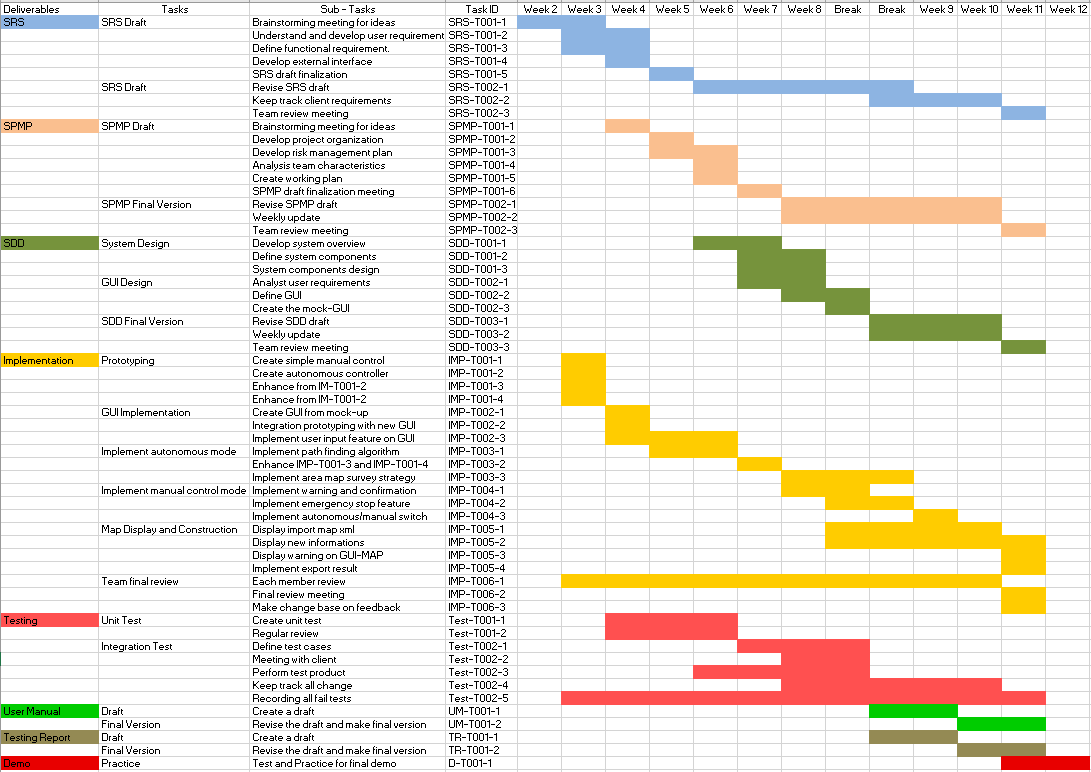
\includegraphics[width=1.5\linewidth]{gantt-chart.PNG}  % created using www.draw.io
	\caption{Gantt Chart To Manage Progress}
	\label{gantt-chart-overview}
\end{figure}

%\section{Gantt Chart - Detailed}
% This looks bad, maybe get rid of this
%\includepdf[pages=-]{gantt-chart-details.pdf}

	
\end{document}
